\documentclass[a4paper, 12pt]{article}
\renewcommand{\baselinestretch}{1.20}
\usepackage{graphicx}
%\usepackage[latin1]{inputenc}
\usepackage{subfigure} %Nur bei Teilbildern (a) (b) (c) notwendig
\usepackage{upgreek}
\usepackage{fancyhdr,a4wide}
%\usepackage{longtable} % nur bei mehrseitigen Tabellen notwendig
%\usepackage{setspace}
%\usepackage{times}
\usepackage{amsmath}
%\usepackage{amsfonts}
%\usepackage{multirow}
\usepackage{hyperref}
\usepackage{listings}


\begin{document}
\hypersetup{colorlinks, linkcolor=red}

\title{\textbf{Distributed ETALIS Manual}}
\author{Jia Ding}
\date{23.03.2013}
\maketitle

\newpage
\tableofcontents

\newpage
\section{About}
\textbf{Distributed-ETALIS} is a distriuted event processing engine. It is based on \textbf{Storm} \cite{web:storm} (a distributed realtime computation system) and \textbf{Kafka} \cite{web:kafka} (a distributed publish-subscribe messaging system). To set up the whole environment please follow the instruction in the next section.

\section{Setting and Build}
Storm cluster mode can only work under Linux, all the developments of distributed-ETALIS are under \textbf{Ubuntu} 12.04-LTS \cite{web:ubuntu}. 

\subsection{Setting up a Storm cluster}
You can read the wiki page of storm (\url{https://github.com/nathanmarz/storm/wiki/Setting-up-a-Storm-cluster}) or read the following subsections.
\subsubsection{Set up a Zookeeper cluster}
Storm uses Zookeeper for coordinating the cluster. Zookeeper is not used for message passing, so the load Storm places on Zookeeper is quite low. Single node Zookeeper clusters should be sufficient for most cases, but if you want failover or are deploying large Storm clusters you may want larger Zookeeper clusters. Instructions for deploying Zookeeper are at (\url{http://zookeeper.apache.org/doc/r3.3.3/zookeeperAdmin.html}).\\

A few notes about Zookeeper deployment:
\begin{itemize}
\item It's critical that you run Zookeeper under supervision, since Zookeeper is fail-fast and will exit the process if it encounters any error case.
\item It's critical that you set up a cron to compact Zookeeper's data and transaction logs. The Zookeeper daemon does not do this on its own, and if you don't set up a cron, Zookeeper will quickly run out of disk space.
\end{itemize}

\subsubsection{Install dependencies on Nimbus and worker machines}
Next you need to install Storm's dependencies on Nimbus and worker machines. These are:
\begin{itemize}
\item \textbf{ZeroMQ 2.1.7}\\
Storm has been tested with ZeroMQ 2.1.7, and is the recommended ZeroMQ release that you install. You can download a ZeroMQ release from \url{http://download.zeromq.org/}. Install ZeroMQ should look something like this:
\begin{lstlisting}
----------------------------------------------------
wget http://download.zeromq.org/zeromq-2.1.7.tar.gz
tar -xzf zeromq-2.1.7.tar.gz
cd zeromq-2.1.7
./configure
make
sudo make install
----------------------------------------------------
\end{lstlisting}

\item \textbf{JZMQ}\\
JZMQ is the Java bindings for ZeroMQ. JZMQ doesn't have any releases, so there is risk of a regression if you always install from the master branch. To prevent a regression from happening, you should instead install from this fork which is tested to work with Storm. Installing JZMQ should look something like this:
\begin{lstlisting}
----------------------------------------------------
git clone https://github.com/nathanmarz/jzmq.git
cd jzmq
./autogen.sh
./configure
make
sudo make install
----------------------------------------------------
\end{lstlisting}
To get the JZMQ build to work, you may need to do one or all of the following:
\begin{itemize}
\item[1)] Install Java dev package
\item[2)] Set JAVA\_HOME environment variable appropriately
\item[3)] Upgrade autoconf on your machine
\item[4)] If you run any errors when running \fbox{./configure}, this thread (\url{http://stackoverflow.com/questions/3522248/how-do-i-compile-jzmq-for-zeromq-on-osx}) may provide a solution.
\item[5)] If you get any errors when running \fbox{make}, this thread (\url{https://github.com/zeromq/jzmq/issues/114}) may provide a solution.
\end{itemize}

\item \textbf{Java 6}

\item \textbf{Python 2.6.6}
\end{itemize}

These are the versions of the dependencies that have been tested with Storm. Storm may or may not work with different versions of Java and/or Python.

\subsubsection{Download and extract a Storm release to Nimbus and worker machines}
Next, download a Storm release and extract the zip file somewhere on Nimbus and each of the worker machines. The Storm releases can be downloaded from \url{https://github.com/nathanmarz/storm/downloads}.

\subsubsection{Fill in mandatory configurations into storm.yaml file}
The Storm release contains a file at \fbox{conf/storm.yaml} that configures the Storm daemons. There's a few configurations that are mandatory to get a working cluster:
\begin{itemize}
\item[1)] \textbf{storm.zookeeper.servers}: This is a list of the hosts in the Zookeeper cluster for your Storm cluster. It should look something like:
\begin{lstlisting}
----------------------------------------------------
storm.zookeeper.servers:
  - "111.222.333.444"
  - "555.666.777.888"
----------------------------------------------------
\end{lstlisting}
If the port that your Zookeeper cluster uses is different than the default, you should set \textbf{storm.zookeeper.port} as well.

\item[2)] \textbf{storm.local.dir}: The Nimbus and Supervisor daemons require a directory on the local disk to store small amounts of state (like jars, confs, and things like that). You should create that directory on each machine, give it proper permissions, and then fill in the directory location using this config. For example:
\begin{lstlisting}
----------------------------------------------------
storm.local.dir: "/mnt/storm"
----------------------------------------------------
\end{lstlisting}

\item[3)] \textbf{java.library.path}: This is the load path for the native libraries that Storm uses (ZeroMQ and JZMQ). The default of "/usr/local/lib:/opt/local/lib:/usr/lib" should be fine for most installations, so you probably don't need to set this config.

\item[4)] \textbf{nimbus.host}: The worker nodes need to know which machine is the master in order to download topology jars and confs. For example:
\begin{lstlisting}
----------------------------------------------------
nimbus.host: "111.222.333.44"
----------------------------------------------------
\end{lstlisting} 

\item[5)] \textbf{supervisor.slots.ports}: For each worker machine, you configure how many workers run on that machine with this config. Each worker uses a single port for receiving messages, and this setting defines which ports are open for use. If you define five ports here, then Storm will allocate up to five workers to run on this machine. If you define three ports, Storm will only run up to three. By default, this setting is configured to run 4 workers on the ports 6700, 6701, 6702, and 6703. For example:
\begin{lstlisting}
----------------------------------------------------
supervisor.slots.ports:
    - 6700
    - 6701
    - 6702
    - 6703
----------------------------------------------------
\end{lstlisting} 
\end{itemize}

\subsubsection{Launch daemons under supervision using storm script and a supervisor of your choice}
The last step is to launch all the Storm daemons. It is critical that you run each of these daemons under supervision. Storm is a fail-fast system which means the processes will halt whenever an unexpected error is encountered. Storm is designed so that it can safely halt at any point and recover correctly when the process is restarted. This is why Storm keeps no state in-process -- if Nimbus or the Supervisors restart, the running topologies are unaffected. Here's how to run the Storm daemons:
\begin{itemize}
\item \textbf{Nimbus}: Run the command "bin/storm nimbus" under supervision on the master machine.
\item \textbf{Supervisor}: Run the command "bin/storm supervisor" under supervision on each worker machine. The supervisor daemon is responsible for starting and stopping worker processes on that machine.
\item \textbf{UI}: Run the Storm UI (a site you can access from the browser that gives diagnostics on the cluster and topologies) by running the command "bin/storm ui" under supervision. The UI can be accessed by navigating your web browser to http://{nimbus host}:8080.
\end{itemize}
As you can see, running the daemons is very straightforward. The daemons will log to the logs/ directory in wherever you extracted the Storm release.

\subsection{Setting up Kafka}
You can download a release of Kafka from \url{http://kafka.apache.org/downloads.html} and unpack it on nimbus and each worker machines. The current stable version is \textit{0.7.2-incubating}.

\subsection{Install SWI-Prolog}
You should follow this link (\url{http://www.swi-prolog.org/build/Debian.html}) to install \textbf{SWI-Prolog}. When you install it, you should remember to enable the \textit{jpl} and \textit{shared} flag.\\
After you install the SWI-Prolog, you should specify the path for the \textbf{JPL} library. For example:
\begin{lstlisting}
----------------------------------------------------
export LD_LIBRARY_PATH=/usr/local/lib/swipl-6.3.10/lib/x86_64-linux
----------------------------------------------------
\end{lstlisting} 


\subsection{Setting up jtalis-distribute}
Jtalis-distribute is a distributed version of Jtalis, which is a Java wrapper for \textbf{ETALIS} \cite{web:etalis} engine. To set up the jtalis-distribute you need to install \textbf{Subversion} and \textbf{Maven}.\\
You should checkout the source from \url{http://etalis.googlecode.com/svn/dEtalis/jtalis-distribute} and build it:
\begin{lstlisting}
----------------------------------------------------
svn chekcout http://etalis.googlecode.com/svn/dEtalis/jtalis-distribute
cd jtalis-distribute/scripts
./build.sh
----------------------------------------------------
\end{lstlisting}


\subsection{Setting up distributed-Etalis}
You should checkout the source from \url{http://etalis.googlecode.com/svn/dEtalis/jtalis-storm-zstream}. Then use \textbf{Maven} to build it.
\begin{lstlisting}
----------------------------------------------------
svn chekcout http://etalis.googlecode.com/svn/dEtalis/jtalis-storm-zstream
cd jtalis-storm-zstream
mvn install
----------------------------------------------------
\end{lstlisting}
In the target folder, you will find \textit{jtalis-storm-zstream-0.0.1-SNAPSHOT.jar}.

\subsection{Run the Demo}
Follow the below instructions to run the demo:
\begin{itemize}
\item[1)] \textbf{Start Zookeeper Server, Storm Nimbus and Storm UI}\\
\begin{itemize}
\item[i)] Login the Storm master node
\begin{lstlisting}
----------------------------------------------------
ssh -i etalis01.pem ubuntu@141.52.160.167
----------------------------------------------------
\end{lstlisting}

\item[ii)] Start Zookeeper Server
\begin{lstlisting}
----------------------------------------------------
cd ~/storm/kafka-0.7.2-incubating-src/
sudo ./bin/zookeeper-server-start.sh config/zookeeper.properties
----------------------------------------------------
\end{lstlisting}

\item[iii)] Start Storm Nimbus
\begin{lstlisting}
----------------------------------------------------
cd ~/storm/storm-0.8.2/
sudo ./bin/storm nimbus
----------------------------------------------------
\end{lstlisting}

\item[iv)] Start Storm UI
\begin{lstlisting}
----------------------------------------------------
cd ~/storm/storm-0.8.2/
sudo ./bin/storm ui
----------------------------------------------------
\end{lstlisting}
After ui started, open a web browser and access the Storm UI with this address (see Fig. \ref{fig:storm_ui}):\\
\url{141.52.160.167:8080}\\
\begin{figure}[!h]
  \begin{center}
    	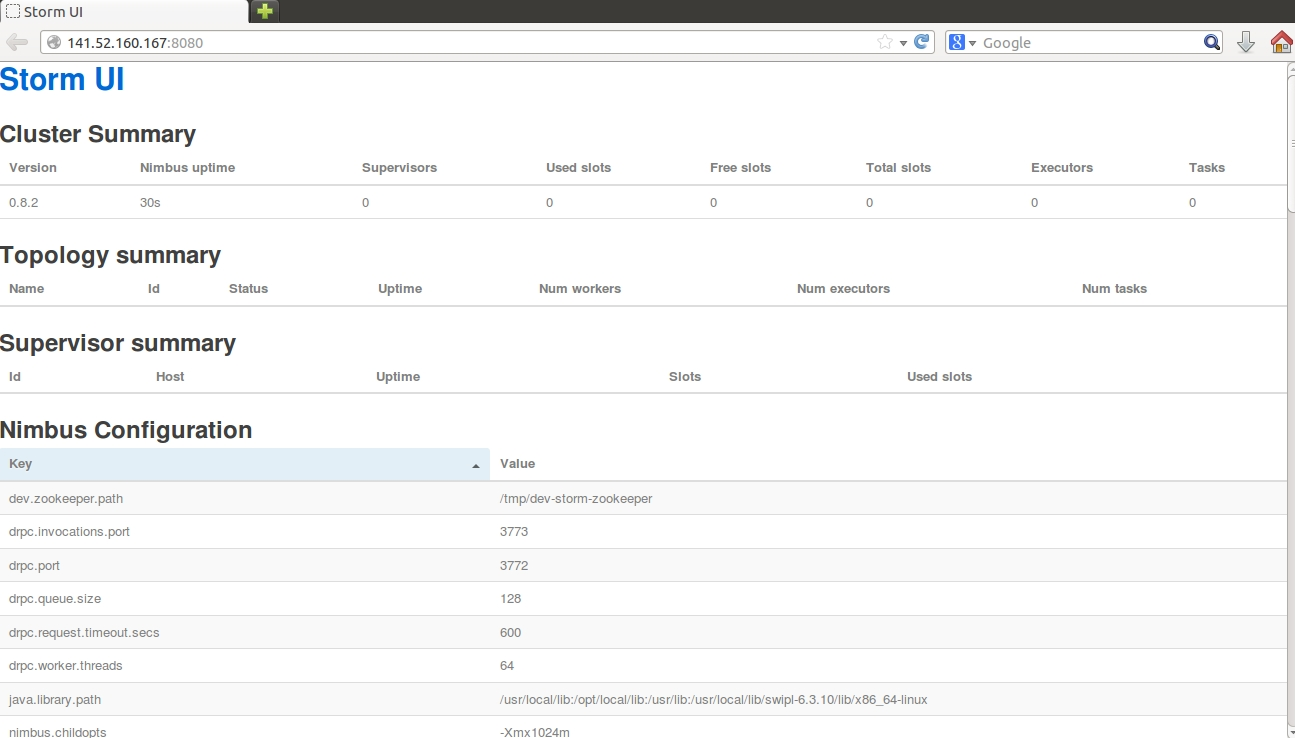
\includegraphics[width=16cm]{photo/storm_ui.jpg}
    	\caption{Storm UI}
    \label{fig:storm_ui}
  \end{center}
\end{figure}
\end{itemize}

\item[2)] \textbf{Start Storm Supervisor daemon}\\
Start Storm Supervisor daemon on each VM.
\begin{lstlisting}
----------------------------------------------------
ssh -i etalis01.pem ubuntu@141.52.160.167
cd ~/storm/storm-0.8.2/
sudo ./bin/storm supervisor

ssh -i etalis02.pem ubuntu@141.52.160.145
cd ~/storm/storm-0.8.2/
sudo ./bin/storm supervisor

ssh -i etalis03.pem ubuntu@141.52.160.146
cd ~/storm/storm-0.8.2/
sudo ./bin/storm supervisor

ssh -i etalis04.pem ubuntu@141.52.160.155
cd ~/storm/storm-0.8.2/
sudo ./bin/storm supervisor

ssh -i etalis05.pem ubuntu@141.52.160.156
cd ~/storm/storm-0.8.2/
sudo ./bin/storm supervisor
----------------------------------------------------
\end{lstlisting}
After start the 5 Supervisor on 5 VM, you can see the this on Storm UI (see Fig. \ref{fig:storm_supervisor}).
\begin{figure}[!h]
  \begin{center}
    	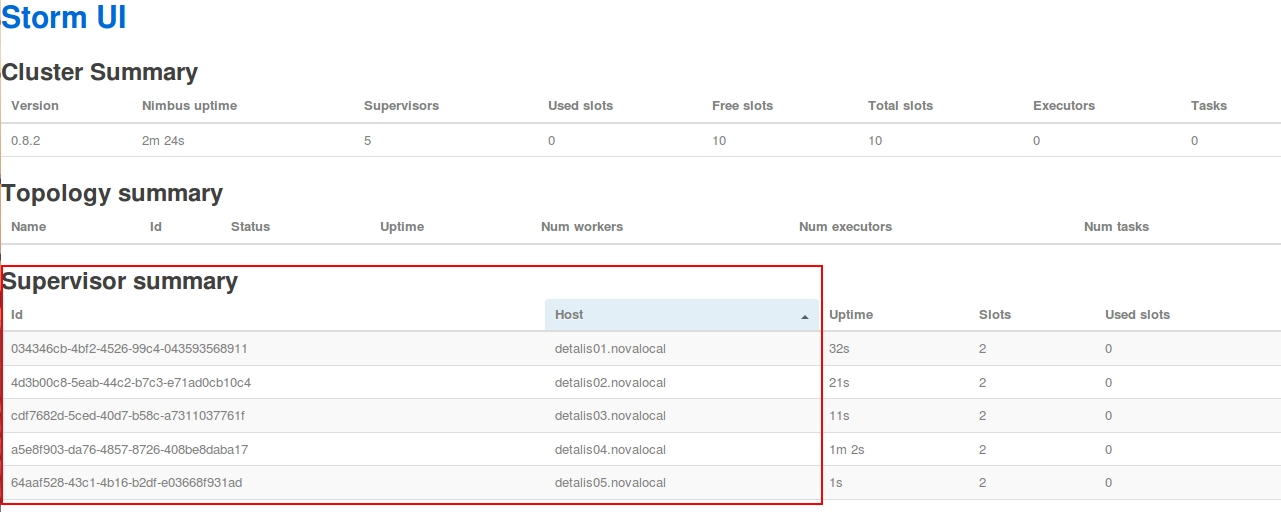
\includegraphics[width=16cm]{photo/storm_supervisor.jpg}
    	\caption{Storm Supervisor}
    \label{fig:storm_supervisor}
  \end{center}
\end{figure}

\item[3)] \textbf{Deploy the Demo Topology}
\begin{itemize}
\item[i)] Compile the source code to .jar file
\begin{lstlisting}
----------------------------------------------------
ssh -i etalis01.pem ubuntu@141.52.160.167
cd dEtalis/
svn update
cd jtalis-storm-zstream/
mvn install
----------------------------------------------------
\end{lstlisting}

\item[ii)] Deploy the Topology to Storm\\
\lstset{
    breaklines     = true,
    stepnumber     = 0,
}
\begin{lstlisting}
----------------------------------------------------
cd ~/storm/storm-0.8.2/
./bin/storm jar ~/dEtalis/jtalis-storm-zstream/target/jtalis-storm-zstream-0.0.1.jar com.jtalis.storm.zstream.topology.ZStreamDemoTopology 10 300 1000
----------------------------------------------------
\end{lstlisting}
\textbf{ZStreamDemoTopology} has 3 parameters:
\begin{itemize}
\item Number of workers: it depends on how many slots that storm has.
\item Atom Events generate time interval: it sets every a period time to generate a atom event.
\item Time Window: it sets the time window of the operator.
\end{itemize}
After you deploy the Topology, you can see it on the Storm UI (see Fig. \ref{fig:storm_topology}).
\begin{figure}[!h]
  \begin{center}
    	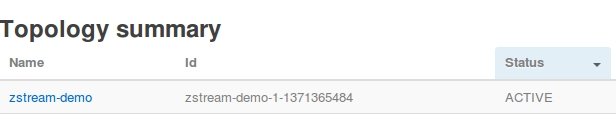
\includegraphics[width=14cm]{photo/storm_topology.jpg}
    	\caption{Storm Topology}
    \label{fig:storm_topology}
  \end{center}
\end{figure}\\
The result is stored by a component of this Topology, the name is \fbox{logBolt}. In Storm UI you can find, on which VM and on which Worker it works (see Fig. \ref{fig:storm_logbolt}). 
\begin{figure}[!h]
  \begin{center}
    	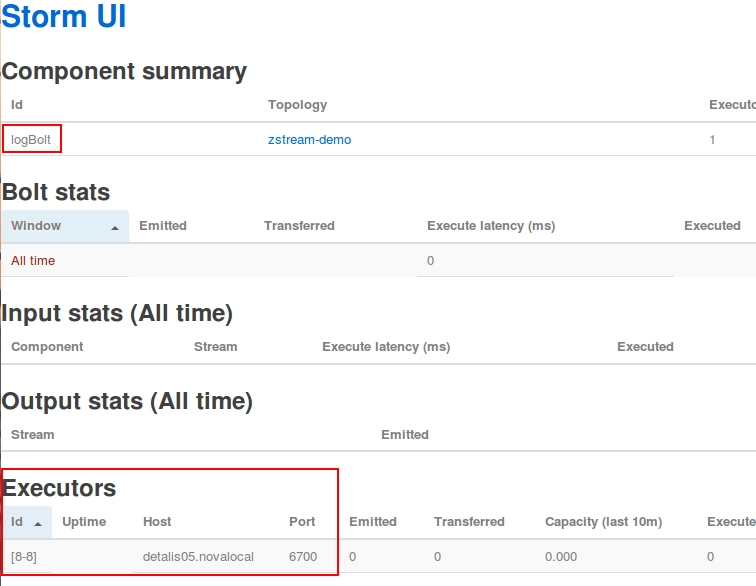
\includegraphics[width=16cm]{photo/storm_logbolt.jpg}
    	\caption{Storm logBolt}
    \label{fig:storm_logbolt}
  \end{center}
\end{figure}\\
Here the logBolt is working on VM 5 and the worker id is 6700. You can login the VM 5 and to check the results (see Fig. \ref{fig:storm_result}).
\begin{figure}[!h]
  \begin{center}
    	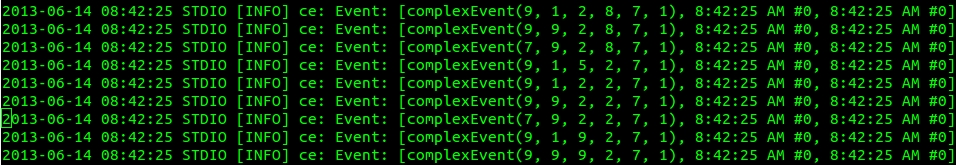
\includegraphics[width=16cm]{photo/storm_result.jpg}
    	\caption{Storm Log}
    \label{fig:storm_result}
  \end{center}
\end{figure}
\begin{lstlisting}
----------------------------------------------------
ssh -i etalis05.pem ubuntu@141.52.160.156
cd ~/storm/storm-0.8.2/logs/
nano worker-6700.log
----------------------------------------------------
\end{lstlisting}

\end{itemize}

\item[4)] \textbf{Undeploy the Demo Topology}
\begin{lstlisting}
----------------------------------------------------
./bin/storm kill zstream-demo
----------------------------------------------------
\end{lstlisting}

\end{itemize}

\newpage
\begin{thebibliography}{9}

\bibitem{web:storm}
  \url{http://storm-project.net/}.
\bibitem{web:kafka}
  \url{http://kafka.apache.org/}.  
\bibitem{web:ubuntu}
  \url{http://www.ubuntu.com/}.  
\bibitem{web:storm_cluster}
  \url{https://github.com/nathanmarz/storm/wiki/Setting-up-a-Storm-cluster}.   
\bibitem{web:etalis}
  \url{http://code.google.com/p/etalis/}.            
\end{thebibliography}
%\bibliographystyle{unsrt}
%\bibliography{website}

\end{document}
